\documentclass[12pt, a4paper]{report}
%%%%%%%%%% Load Package %%%%%%%%%%%
\usepackage[top=3.0cm,bottom=2.0cm,left=3cm,right=3cm]{geometry}
\usepackage{fontspec}
\usepackage[noblocks,affil-it]{authblk}
\usepackage[colorlinks = true,
	    	linkcolor = cyan,
            citecolor = blue,
            anchorcolor = blue]{hyperref}
\usepackage{listings}
\usepackage{booktabs}
\usepackage{titlesec}
\usepackage{chngpage}
\usepackage{array}
%%%%%%%%%% Set Format %%%%%%%%%%%%%%
\setmainfont{Times New Roman}
\newfontfamily{\C}{Consolas}
\newfontfamily{\tb}{Times New Roman Bold}
\newfontfamily{\ti}{Times New Roman Italic}

\lstset{basicstyle=\C,
  showstringspaces=false,
  commentstyle=\color{red},
  keywordstyle=\color{blue},
  backgroundcolor=\color[rgb]{1.0,1.0,0.95},
}
\titleformat{\chapter}{\Huge\bfseries}{\thechapter}{1em}{}
%%%%%%%%%% First Page %%%%%%%%%%%%%%
\title{Seispy\\User Manual of Receiver Functions}
\author[1,*]{Mijian Xu}
\affil[1]{\small School of Earth Science and Engineering, Nanjing University}
\affil[*]{\small Email: gomijianxu@gmail.com}

\begin{document}
\maketitle
\tableofcontents

%===================================%
%------------ Chapter 1 ------------%
%===================================%
\chapter{Introduction}
Seispy is a Python package to process Seismic waveform and receiver functions. This package not only provide a python module but also include scripts to batch receiver functions. This package can only support Linux and Mac OSX platform with Python 3.x (I am not sure the compatibility with the Python 3.5.x+). It is distributed under the GNU General Public License Version 3 (GPLv3) as published by the Free Software Foundation (\url{http://www.gnu.org/licenses/gpl.html}).

%===================================%
%------------ Chapter 2 ------------%
%===================================%
\chapter{Installation}

%----------- Section 2.1 -----------%
\section{Dependencies}
Seispy depends on standard libraries of Python 3.x and the Obspy module (\url{http://docs.obspy.org}). Moreover, This package require GMT 5.x (\url{http://gmt.soest.hawaii.edu}) in plotting receiver functions.

%----------- Section 2.1 -----------%
\section{Installation}
\begin{enumerate}
\item Install Obspy and GMT.
\item Download Seispy. Opening terminal, run the following commands:
\begin{lstlisting}[language=bash]
git clone https://github.com/xumi1993/seispy.git
\end{lstlisting}
\item Install seispy by running following commands:
\begin{lstlisting}[language=bash]
cd seispy
python setup.py install
\end{lstlisting}
\item If the scripts are required, please add executable scripts to environment path. The executable scripts include {\C pickrf.py, pickrf\_R.py, updateCatalog.py} and {\C makeRF4station.py}, which used to calculate and filter receiver functions in a batch.
\end{enumerate}


\chapter{Tutorial of calculating receiver functions}
\section{A function of iterative deconvolution}
Using this {\C seispy.decov} to calculate receiver functions by iterative deconvolution.
\subsection{decovit}
\begin{lstlisting}
RFI, RMS, IT = seispy.decov.decovit(UIN,WIN,DT,NT,TSHIFT,
		F0,ITMAX,MINDERR)
\end{lstlisting}
\paragraph{\tb Parameters:}
\begin{description}
\item UIN = numerator (radial for PdS in {\C numpy.ndarray})
\item WIN = denominator (vertical component for PdS in {\C numpy.ndarray})
\item DT = sample interval (s)
\item NT = number of samples
\item TSHIFT = Time until beginning of receiver function (s)
\item F0 = width of gaussian filter
\item ITMAX = max \# iterations
\item MINDERR = Min change in error required for stopping iterations.
\end{description}
\paragraph{Output}
\begin{description}
\item RFI = receiver function ({\C numpy.ndarray}).
\item RMS = Root mean square error for predicting numerator after each iteration.
\item IT = number of iterations.
\end{description}

\subsection{gaussFilter}
Design Gauss filter.
\begin{lstlisting}
gauss = seispy.decov.gaussFilter( dt, nft, f0 )
\end{lstlisting}
\paragraph{Parameters:}
\begin{description}
\item dt = sample interval (s)
\item nft = number of samples
\item f0 = width of gaussian filter
\end{description}
\paragraph{Output:}
\begin{description}
\item gauss = series of gauss filter in {\C numpy.ndarray}
\end{description}

\section{Calculating receiver function in a batch}
\subsection{Usage}
The {\C makeRF4station.py} is a script to calculate receiver function in a batch.
\begin{lstlisting}
python makeRF4station.py -Sstation \
	-Yyearmin/monthmin/daymin/yearmax/monthmax/daymax\
	-Cchannel [-T[+E|+N]] [-r] paraRF.cfg
\end{lstlisting}
\subsection{Synopsis}
\begin{description}
\item {\tb -S} The station name. It must be same as the directory name, which include original data of SAC format.
\item {\tb -Y} A rough date range during this operation.
\item {\tb -C} A component name in SAC file name (e.g., {\ti BHZ, HHZ, 1}.)
\item {\tb -T} Attach {\tb +E} to switch east component sign. Attach {\tb +N} to switch north component sign.
\item {\tb -r} Only calculate radial receiver functions
\item {\tb paraRF.cfg} Parameters of calculating receiver functions (see Table \ref{tab1}).
\begin{table}[h]
\caption{Options in config file}
\centering
\begin{tabular}{|p{.2\textwidth}|m{.7\textwidth}|} \toprule[1.5 pt]
Option & Function \\ \midrule[1 pt]
{\C data\_path} & Directory of original data\\
{\C out\_path} &  Data after cutting by time window\\
{\C RF\_path} & Directory of receiver functions\\
{\C image\_path} & Directory of Figures\\
{\C evt\_list} & Directory of Catalog\\ \midrule[1 pt]
{\C gate\_mw} & Low boundary of magnitude\\
{\C gate\_dis1} & Low boundary of epicenteral distance\\
{\C gate\_dis2} & High boundary of epicenteral distance\\
{\C time\_before} & Low boundary of time window\\
{\C time\_after} & High boundary of time window\\
{\C tolerance} & This value in seconds will define the time window within which the program will try to associate a seismic file to an event file.\\
{\C offset} & A time duration between the event time and the starting time of your seismograms.\\
{\C gate\_noise} & A threshold value in SNR analysis.\\
{\C gauss} & Gauss factor.\\
{\C freqmin} & Low cut-off frequency of a filter before calculating receiver function.\\
{\C freqmax} & High cut-off frequency of a filter before calculating receiver function.\\
{\C sampling} & time interval in second, which the program will resample waveforms to this sampling rate.\\
\bottomrule[1.5 pt]
\end{tabular}
\label{tab1}
\end{table}
\end{description}

\subsection{Example}
\begin{lstlisting}
python makeRF4station.py -SNJ2 -Y2015/1/1/2015/12/1 -CBHZ paraRF.cfg
python makeRF4station.py -SNJ2 -Y2015/1/1/2015/12/1 -CBHE -T+E paraRF.cfg
\end{lstlisting}
\subsection*{Note:}
\begin{enumerate}
\item This program will calculate P-wave arrival time automatically. Therefore, locations of station must be written in SAC header value.
\item The {\C tolerance} value in seconds will define the time window within which the program will try to associate a seismic file to an event file, by using either its name or the information contained in the header. It is up to the user to find the best compromise: a value too small will let orphans and a value too large will bring confusion since several files could be associated to a seismic event ({\ti See Splitlab User Manual}).
\item The {\C offset} is the time duration between the event time and the starting time of your seismograms. Ideally, this offset should be identical to the "request start time" defined in the previous window but the data management center may have sent you data beginning later than requested. The offset value represents this difference ({\ti See Splitlab User Manual}).
\end{enumerate}
\section{Filter receiver functions manually}
{\C pickrf.py/pickrf\_R.py} are GUI scripts to process receiver functions after running {\C makeRF4station.py}
\subsection{Usage}
\begin{lstlisting}
python pickrf.py -Sstation paraRF.cfg
\end{lstlisting}
\subsection{Synopsis}
All of these arguments are same as that in {\C makeRF4station.py}.
\subsection{Interface}
Figure \ref{fig:pick} shows this GUI interface 
\begin{figure}[htbp]
  \centering
  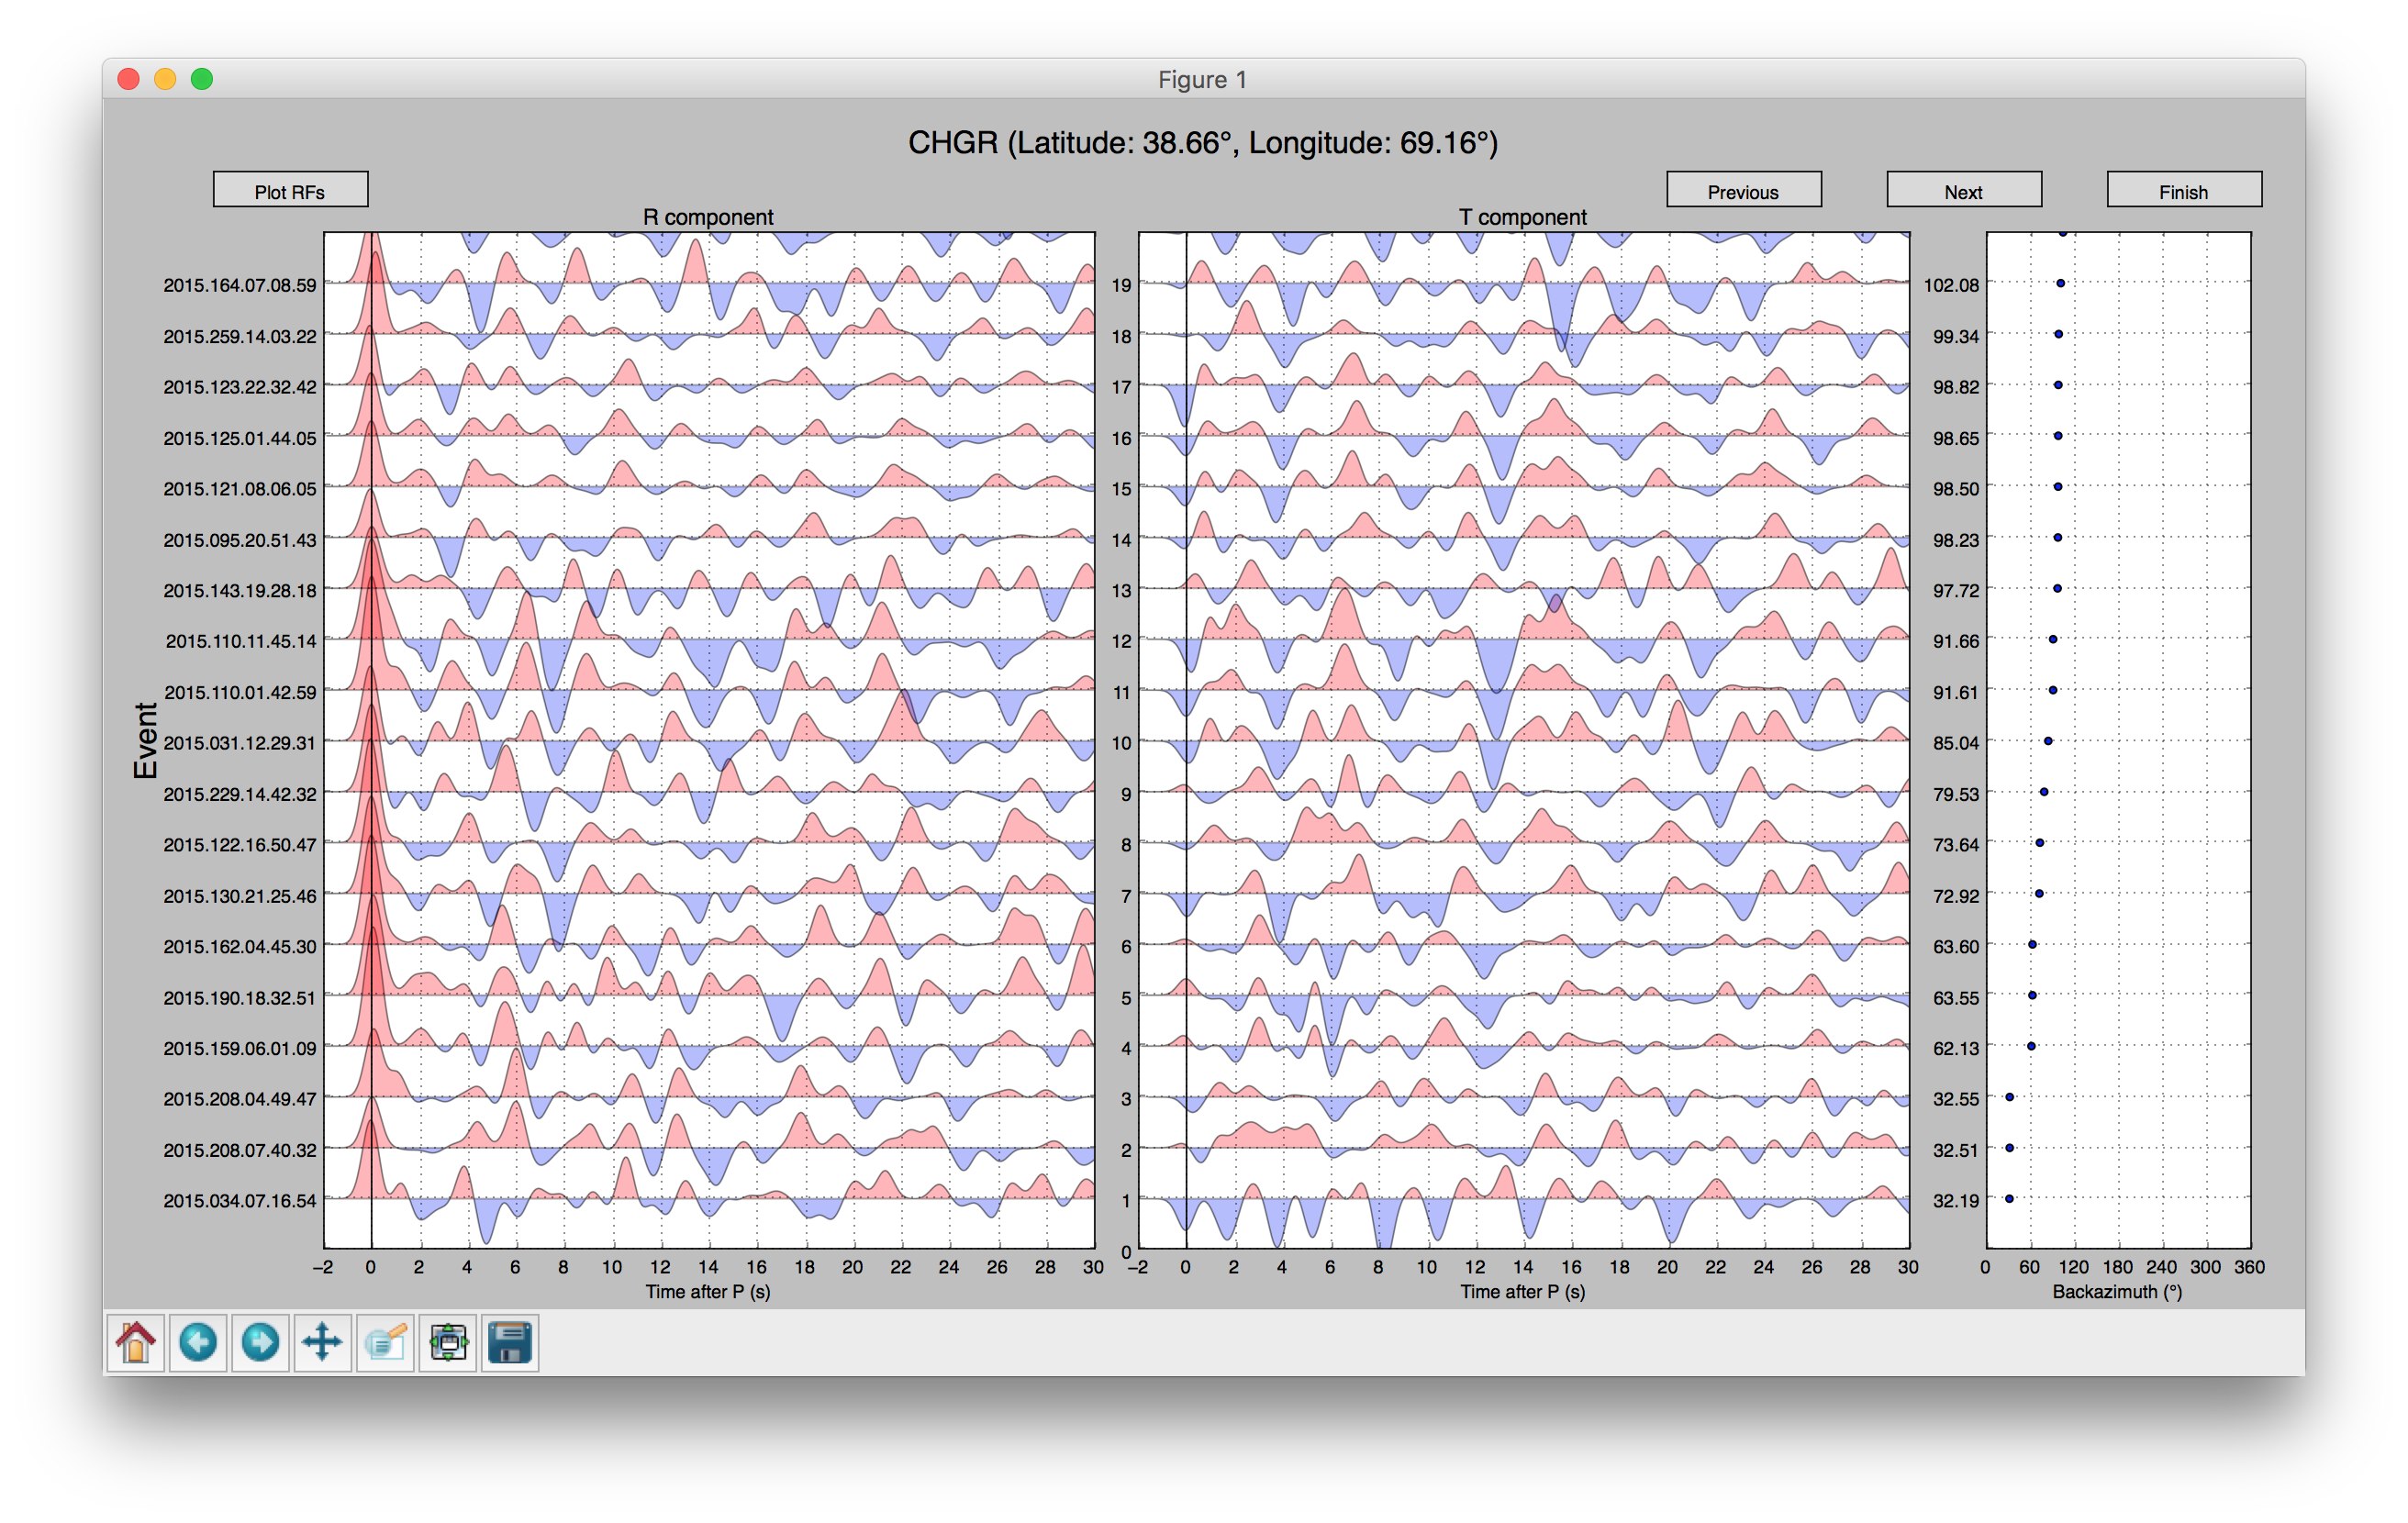
\includegraphics[width= 1\textwidth]{./snapshot.png}
  \caption{GUI Interface to process receiver functions.}\label{fig:pick}
\end{figure}

\end{document}





